\chapter{Securities Fraud, Event Studies and Prices as Evidence}
\label{ch:securities}

\section{Markets as witnesses}

In securities litigation, the market is a witness. When a company makes a false statement about its business, investors who trade on the market price are affected even if they never read the statement, because the price reflects it. When the truth emerges, the price falls, and the fall measures, at least approximately, the value of the misinformation. Courts in the United States have built the law of securities fraud class actions around this idea, and the statistical tool that implements it, the event study, has become one of the most frequently litigated statistical methods in American courts. This chapter explains the legal framework, the method and its Bayesian reinterpretation, and then turns to an English case that raised related questions in a different procedural setting: the Autonomy litigation, whose central figure built a company on Bayesian inference.\index{securities fraud}\index{event study}

\section{Fraud on the market}

\subsection{Basic v Levinson}

Rule 10b-5 under the Securities Exchange Act of 1934 prohibits material misstatements in connection with the purchase or sale of securities. A private plaintiff must prove, among other things, reliance on the misstatement. In a class action involving thousands of investors, individual proof of reliance would be impossible. In \emph{Basic Inc v Levinson} the Supreme Court in 1988 adopted the fraud on the market presumption: in an efficient market, the price reflects all public information, including misstatements, so an investor who trades at the market price relies on the misstatement through the price \citep{basic1988}. The presumption can be rebutted by showing that the misstatement did not affect the price.\index{Basic v Levinson}\index{fraud on the market}

\subsection{Price impact}

In \emph{Halliburton Co v Erica P. John Fund}, the second time the case reached the Supreme Court, the Court in 2014 declined to overrule \emph{Basic} but held that defendants may rebut the presumption at the class certification stage by showing that the alleged misrepresentation had no price impact \citep{halliburton2014}. In \emph{Goldman Sachs Group v Arkansas Teacher Retirement System} the Court in 2021 held that courts must consider the generic nature of a misrepresentation in assessing price impact, and that when a generic statement such as a commitment to integrity is alleged to have maintained an inflated price, which then fell on a specific corrective disclosure, the mismatch between the generic statement and the specific disclosure undermines the inference of price impact \citep{goldman2021}. Price impact is now a central battleground, and it is fought with event studies.\index{price impact}

\subsection{Loss causation}

A plaintiff must also prove loss causation: that the misrepresentation, not other factors, caused the loss. In \emph{Dura Pharmaceuticals v Broudo} the Court held in 2005 that an inflated purchase price alone does not establish loss; the plaintiff must show that the misrepresentation caused an economic loss, ordinarily by showing that the price fell when the truth was revealed \citep{dura2005}. Again the evidence is an event study around the corrective disclosure.

\section{The event study}

\subsection{The method}

An event study estimates how much of a stock's return on a given day is attributable to company specific news. The analyst estimates a model of normal returns, typically a market model relating the stock's return to the return on a market index and perhaps an industry index, over a period without unusual events:
\begin{equation}
r_t = \alpha + \beta\, m_t + \epsilon_t, \qquad \epsilon_t\sim N(0,\sigma^2).
\end{equation}
On the event date, the abnormal return is the difference between the actual return and the return predicted by the model, $a_0 = r_0 - \hat\alpha - \hat\beta m_0$. Its significance is assessed by dividing by $\hat\sigma$, giving approximately a $t$ statistic; a value beyond about two is conventionally treated as statistically significant. Cumulative abnormal returns sum abnormal returns over a window. Figure~\ref{fig:event} shows a simulated corrective disclosure against a background of normal variation.

\begin{figure}[t]
\centering
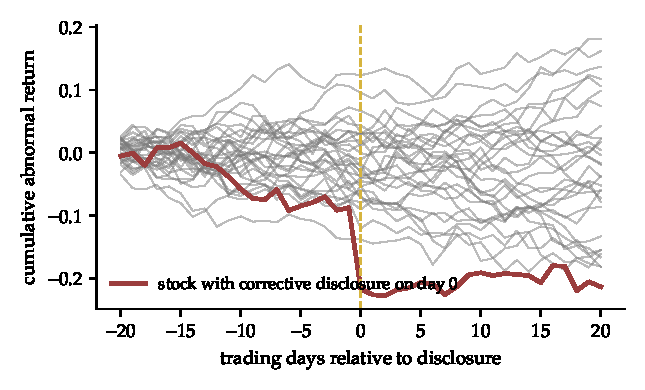
\includegraphics[width=\linewidth]{fig_event}
\caption{Cumulative abnormal returns for a simulated stock with a corrective disclosure on day zero, against thirty simulated paths with no event. Illustrative.}
\label{fig:event}
\end{figure}

\subsection{Problems in court}

Event studies in litigation face well known problems. Single firm, single day tests have low power: a stock with daily volatility of two per cent cannot reliably reveal a price impact of less than about five or six per cent. Volatility changes around news, so the estimation period's $\sigma$ may understate the event day's. Multiple pieces of news on the same day must be disentangled. And the significance threshold, borrowed from academic practice, has no legal warrant: a p value of five per cent is a convention, not a standard of proof. Fisch, Gelbach and Klick have argued that courts misuse significance tests in this context, treating failure to reject the null of no impact as proof of no impact, and treating the five per cent threshold as if it were the civil standard \citep{fox2018}.

\section{A Bayesian event study}

\subsection{From significance to probability}

The legal question in a price impact dispute is whether the misrepresentation or the corrective disclosure moved the price. A Bayesian answer gives the posterior probability that the abnormal return on the event day reflects a genuine price reaction, and the posterior distribution of its size. Let $\delta$ be the true price impact. The observed abnormal return is $a_0 = \delta + \epsilon_0$. With a prior on $\delta$ and the normal model for $\epsilon_0$, the posterior follows directly. To obtain a probability that there was any reaction at all, the prior must place positive probability $p$ on $\delta=0$ (no impact) and spread the remaining $1-p$ over nonzero impacts, as in Question 1; under a purely continuous prior the posterior probability of exactly zero impact is itself zero, and the useful summary is instead the posterior probability that $|\delta|$ exceeds a legally material size. The prior should reflect what is known about price reactions to comparable disclosures: most company news days produce small abnormal returns, and a minority produce large ones.

\subsection{Heavy tailed priors}

The shape of the prior matters. A normal prior shrinks every estimate toward zero by the same proportion, so a large observed abnormal return is shrunk as much, proportionally, as a small one. A heavy tailed prior (a continuous prior, so the question it answers is about the size of the impact), such as a Cauchy or a horseshoe, shrinks small estimates strongly toward zero while leaving large ones nearly untouched \citep{carvalho2010}. Figure~\ref{fig:heavytail} compares the two. For event studies, a heavy tailed prior is a natural modelling choice, since news day returns are mostly small with a few large ones (event day returns are reported to be fat tailed), and it gives answers that match the intuition, given the prior: a large drop on a corrective disclosure day almost certainly reflects a genuine reaction of material size, while a small drop is likely noise.\index{heavy tailed prior}\index{horseshoe prior}

\begin{figure}[t]
\centering
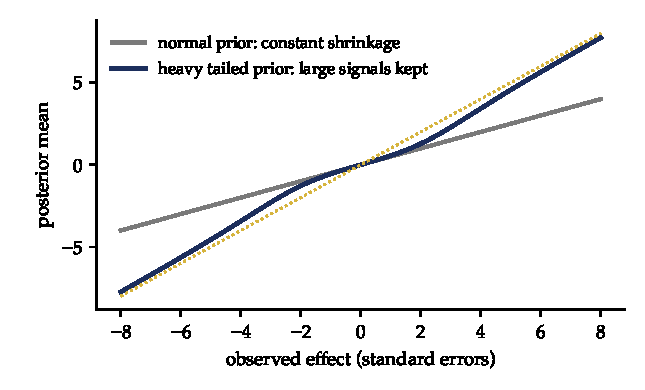
\includegraphics[width=\linewidth]{fig_heavytail}
\caption{Posterior mean of a true effect as a function of the observed effect, under a normal prior and under a heavy tailed (Cauchy) prior, with unit noise. The heavy tailed prior shrinks small observations strongly and large ones hardly at all.}
\label{fig:heavytail}
\end{figure}

Polson and Scott used the same reasoning to screen firms for sustained superior performance, in \emph{Good, great, or lucky?} \citep{polson_scott_lucky}. When many firms are evaluated, most have true excess performance near zero, and a few may be genuinely superior. A heavy tailed prior on performance shrinks the many lucky records toward zero while preserving the few that are too large to be luck. The legal parallels are direct: the same method separates genuine price reactions from noise in event studies, and genuine skill from chance in the games of Chapter~\ref{ch:kadane}.

\subsection{Combining evidence across events}

Price impact often turns on several dates: the original misstatement, partial corrections, and a final disclosure. A hierarchical model treats the impacts on these dates as related, sharing information about the size of the inflation, and estimates them jointly. If the inflation was introduced by a misstatement and removed by several partial disclosures, the impacts should sum, approximately, to the total inflation. This constraint, imposed through the model, strengthens inference about each date. It also addresses the \emph{Goldman} mismatch problem: if a generic statement is alleged to have maintained inflation that a specific disclosure removed, the model must explain why the generic statement carried the specific information, and the prior for that link can be argued about explicitly.

\section{Damages}

Damages in a fraud on the market case are typically measured by the inflation in the price at each purchase date, the difference between the price paid and the price that would have prevailed without the fraud, limited by the decline when the truth emerged. The inflation ribbon, the path of inflation over the class period, is estimated from the event study. Its uncertainty is substantial, and Bayesian methods report it as a posterior distribution rather than a point estimate. In settlement negotiations, which resolve almost all such cases, the posterior distribution of damages, combined with the probability of liability, gives each side's expected value of trial; Chapter~\ref{ch:becker} develops the settlement model that uses it.

\section{Autonomy: Bayes on trial}

\begin{casebox}{ACL Netherlands v Lynch [2022] EWHC 1178 (Ch)}
In 2011 Hewlett Packard acquired Autonomy, a British software company founded by Mike Lynch, for about eleven billion dollars. Autonomy's technology for searching unstructured information was built on Bayesian inference and Shannon's information theory. A year later HP wrote down the value of Autonomy by about nine billion dollars, attributing much of the write down to accounting improprieties. HP's subsidiaries sued Lynch and Autonomy's former finance director in the English High Court under the Financial Services and Markets Act 2000 and in deceit. After a trial that ran from March 2019 to January 2020 and that the judge described as amongst the longest and most complex in English legal history, Mr Justice Hildyard found in 2022 that the defendants had fraudulently inflated Autonomy's reported revenues and that the claimants had succeeded in substantial part \citep{autonomy2022}. Damages were later assessed in a separate judgment at about \pounds 646 million, far below HP's original claim of up to \$5 billion \citep{autonomy2025}. In the United States, Lynch was tried on criminal fraud charges and acquitted by a jury in June 2024. Two months later he died when his yacht, named \emph{Bayesian}, sank off Sicily.
\end{casebox}

\subsection{Different courts, different standards}

The Autonomy litigation shows, like Simpson in Chapter~\ref{ch:classic}, how different standards and procedures can produce different outcomes on overlapping facts. The English civil court applied the balance of probabilities, after a trial in which a single judge heard months of evidence and gave a reasoned judgment of great length. The American criminal jury applied proof beyond reasonable doubt and gave an unreasoned verdict. A posterior probability of fraud somewhere between one half and the criminal threshold would produce exactly these outcomes. The cases also differed in their evidence and in what had to be proved: the English claim under section 90A of the Financial Services and Markets Act turned on the knowledge of persons discharging managerial responsibilities and on the claimants' reliance on published information, while the American prosecution had to prove criminal intent in respect of particular counts.

\subsection{Section 90A and reliance}

Section 90A and Schedule 10A of the Financial Services and Markets Act create liability of an issuer for misleading statements in published information, where a person discharging managerial responsibilities knew the statement was untrue or misleading or was reckless as to that, and the claimant acquired securities in reliance on the information. Unlike American law, English law has not adopted a fraud on the market presumption, and claimants must show reliance on the published information. Claimants in several recent English securities actions have argued that reliance on the market price should suffice, and defendants that individual reliance must be proved. The point is unsettled: in \emph{Allianz Funds v Barclays} the High Court held that reliance under section 90A is the common law deceit test and struck out claims based on reliance on the market price \citep{allianz2024}, but in \emph{Persons Identified in Schedule 1 v Standard Chartered} another High Court judge declined to follow that approach and allowed passive investor claims to go to trial \citep{stanchart2025}. In Bayesian terms, the question is whether the misstatement's effect on the claimant's decision ran through the claimant's own reading of the information, which must be shown individually, or through the price, which can be shown for all buyers at once with an event study. The answer bears on whether securities class actions are viable in England on the American scale, together with the absence of an opt-out regime and the funding and costs rules.

\subsection{The valuation question}

The deeper Bayesian question in Autonomy was what HP would have paid had it known the truth. That is a counterfactual decision, like the insurer's counterfactual premium under the Insurance Act in Chapter~\ref{ch:misrep}. The claimants' loss under the Act was the difference between what they were persuaded to pay and what they would have been persuaded to pay with accurate information, not the whole write down, which also reflected HP's own management of the business after acquisition and changes in market conditions. Separating the effect of the misrepresentation from these other causes required a model of how a buyer values a software company from its revenues, margins and growth, and of how the restated figures would have changed that valuation. The gap between the headline write down and the loss recoverable on this measure illustrates how much of a headline loss can be attributed to causes other than the fraud once the counterfactual is modelled.

\section{Prices as evidence elsewhere}

Market prices are evidence in many other legal contexts. Chapter~\ref{ch:bankruptcy} showed their use in solvency disputes. In appraisal proceedings in Delaware, which determine the fair value of shares of dissenting shareholders in a merger, the Delaware Supreme Court has emphasised the probative value of the deal price when the sale process was sound, and has said that the unaffected market price may be informative in an efficient market but is not necessarily an exclusive indicator \citep{aruba2019}. In antitrust, prices before and during an alleged cartel are compared to estimate overcharges. Prediction market prices are increasingly cited as evidence of expectations. In each case the Bayesian questions are the same: what information does the price aggregate, how reliable is that aggregation, what else moves the price, and how should the price be combined with other evidence?

\section*{Notes and Questions}
\addcontentsline{toc}{section}{Notes and Questions}
\begin{enumerate}[label=\arabic*.]
\item A stock has daily residual volatility of two and a half per cent. On a corrective disclosure date, its abnormal return is minus four per cent. Compute the $t$ statistic. With a prior that ninety per cent of disclosure days have no impact and ten per cent have an impact distributed normally with standard deviation eight per cent, compute the posterior probability of a genuine impact.
\item Explain why a single firm event study has low power, and why failure to find a significant abnormal return does not prove absence of price impact.
\item Compare a normal and a Cauchy prior for a disclosure that produced an abnormal return of ten standard errors. What does each imply about the true impact?
\item In \emph{Goldman}, the alleged misstatements were generic statements about conflicts of interest. Formalise the mismatch argument as a statement about the likelihood that a generic statement carried the information later disclosed.
\item Should English law adopt a fraud on the market presumption for claims under section 90A? Frame your answer in terms of the cost of proving individual reliance and the accuracy of price based inference.
\item Why might a civil court find fraud on the balance of probabilities and a criminal jury acquit on overlapping facts? Use the Autonomy litigation to illustrate.
\end{enumerate}

\section*{Further reading}
The Supreme Court's decisions in \emph{Basic}, \emph{Halliburton} and \emph{Goldman} \citep{basic1988,halliburton2014,goldman2021}; Fisch, Gelbach and Klick on event studies in court \citep{fox2018}; Carvalho, Polson and Scott on the horseshoe prior \citep{carvalho2010}; Polson and Scott on screening firms for sustained performance \citep{polson_scott_lucky}.
